\chapter{Conclusion and future work}
\label{chap:future}

\section{Summary}
This thesis proposes a novel method for recognizing entailment using semantic
graphs and apply it to the 2018 Semeval task on Machine
Comprehension (MC). First, a brief overview of the field of natural language processing is given focusing on real life applications, that are in need of the NLP technologies. Then the topic of computational semantics was discussed in details, focusing on one-two major tasks, like question-answering or information retrieval. After that the formalism of 4lang was presented with examples, and the method of expansion was discussed. After simple yet a strong baseline method was presented for measuring
textual entailment and its application to the comprehension task, followed by an introduction to the field of deep learning. Finally the last chapter reports the results of applying the baseline method
to the MC task and also of using it as an extra feature in the neural network
based \texttt{Yuanfudao} system.

\section{Future work}
Our results are quite promising, but
further experiments are required to explore whether our enhancements can
improve the top-ranking system that also employs
pretraining and an ensemble of multiple models.
We also plan to incorporate sentence-level support
into the system as a more direct application of our
baseline. 


\begin{figure*}[h]
	\centering
	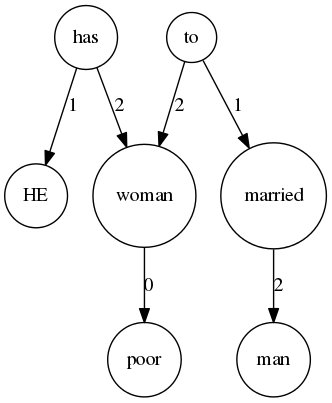
\includegraphics[scale=0.4]{figures/mypoorabs}
	\caption{Example of the \textit{"abstract"} method}
	\label{fig:mypoorabs}
\end{figure*}

We also have some experiments with defining new additional rules added to the \textbf{4lang} parser, that could potentially be giving us a more abstract and simpler definitions than the \textit{expansion} method. Let us look back the sentence "My poor wife" and the expanded graph shown in Figure \ref{fig:mypoorexpanded}. In this example if we look at the edge \textbf{wife $\xrightarrow0$ woman} we can make an assumptions, that native speakers can easily make using simple inference rules \cite{Kovacs:2018}. In our example, within the boundaries of the sentence we can use the concept \textbf{woman} instead of the concept \textbf{wife}. Using this simple rule we can reduce our graph to a simpler definition shown in Figure \ref{fig:mypoorabs}.

\subsection{Interpreted Regular Tree Grammar}
We recently started experimenting with Interpreted Regular Tree Grammars \cite{Koller:2011} (IRTG) that we could also use to construct \textbf{4lang} graphs, since they implement graph transformations, so graph grammars can be used. And by modifying the rules of the grammar, we can also accomplish the \textit{expand} functionalities and we also can define inference rules. These experiments are not yet perfect, but this approach shows great potential. See the phrase \textit{"Ordinary email"} represented in Figure~\ref{fig:irtg}.

The base of this approach is to define grammar files where we describe the rules using multiple graph, tree or string algebras. This allows us to use it as a graph rewriting grammar file which we can use to transcribe for example a universal dependency graph to a \texttt{4lang} graph.

We used an already functioning grammar that defined the relationships between universal dependencies and \texttt{4lang} graphs and modified it to incorporate the definition of the words also \cite{AcsEvelin:2018}.

\begin{figure*}[h]
	\centering
	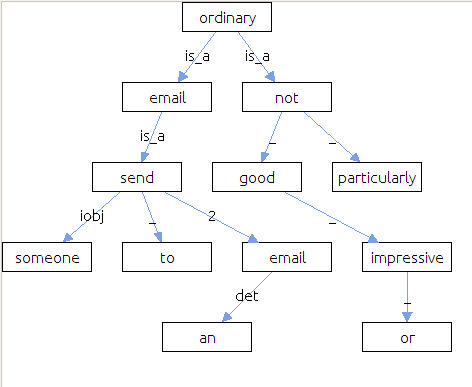
\includegraphics[scale=0.4]{irtg.jpg}
	\caption{Example of the \textit{"expand"} method using IRTG}
	\label{fig:irtg}
\end{figure*}